\chapter{Mikrogesten}

Die grundsätzliche Idee zur Handschrifterkennung ist die Unterteilung der Schrift in sogenannte Mikrogesten. Eine Mikrogeste ist eine simple Bewegung, die beim Schreiben ausgeführt wird. Jeder Buchstabe soll dann aus solchen Mikrogesten aufgebaut werden können. 
Es ist nun natürlich möglich diese Mikrogesten auf beliebige Art zu definieren. Die Hauptkriterien sind, dass die Gesten so einfach wie möglich sein sollen (Für eine optimale Erkennung) und sich untereinander möglichst stark unterscheiden. Je weniger solche Gesten man braucht, desto besser. Man kann jedoch nicht beliebig grobe Gesten wählen, da immer noch alle möglichen Zeichen einzigartig aus solchen Gesten zusammen gebaut werden müssen.

\begin{figure}[h!]
  \centering
    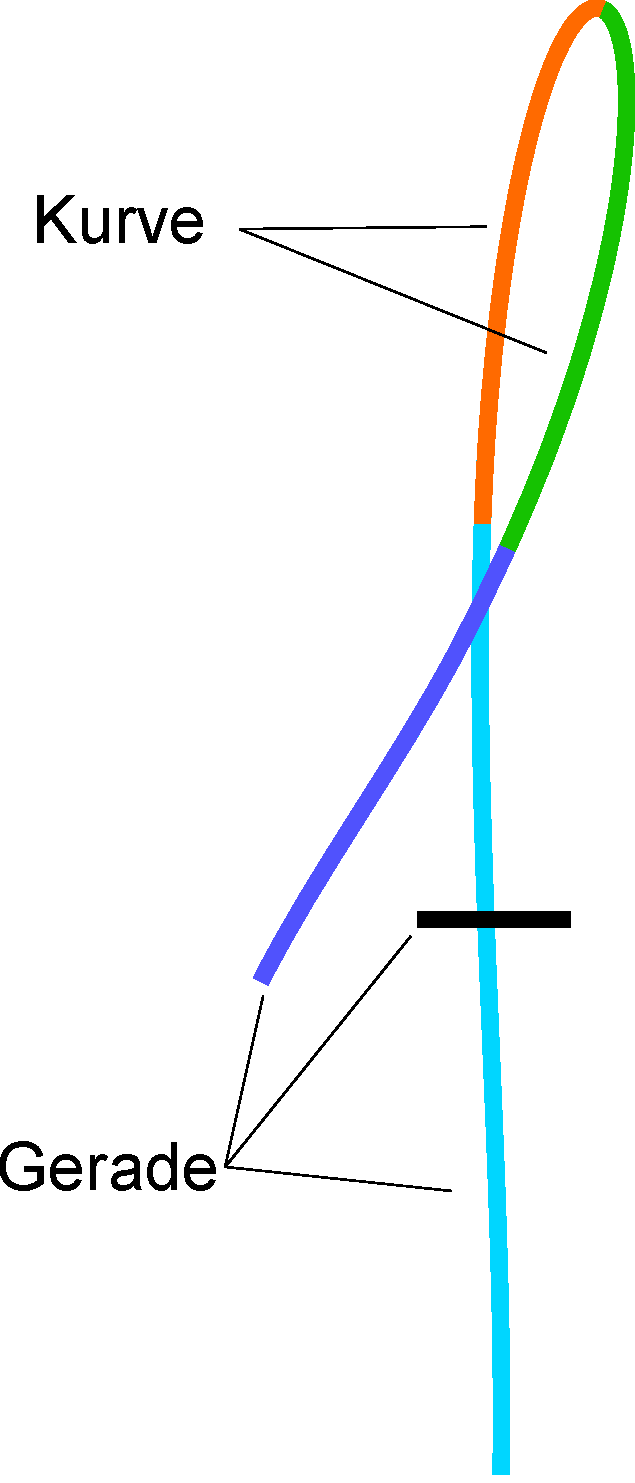
\includegraphics[width=0.2\textwidth]{./img/mikrogesten_beispiel.pdf}
  \caption{Beispiel für die Auftrennung des Buchstaben 'f' in Mikrogesten.}
  \label{mikrogeste_beispiel}
\end{figure}

In der Abbildung \ref{mikrogeste_beispiel} sieht man eine mögliche Aufteilung des Buchstaben 'f' in die Mikrogesten \emph{Kurve} und \emph{Gerade}. Der Buchstabe wird also durch die Abfolge Gerade-Kurve-Kurve-Gerade-Gerade definiert. Nur zwei Mikrogesten sind allerdings zu wenige um alle Zeichen eindeutig abzubilden.

\section{Eigenschaften}
Die Mikrogesten müssen genau definiert werden und können mehr als eine Eigenschaft besitzen:

\subsubsection{Form}
Es ist naheliegend die Mikrogesten hauptsächlich anhand ihrer Form zu unterscheiden. Diese Eigenschaft reicht jedoch nicht, um alle Buchstaben einzigartig zu beschreiben. Zum Beispiel könnte ein 'b' und ein 'p' beides als Gerade-Kreis beschrieben werden. 

\subsubsection{Ausrichtung}
Die Ausrichtung kann auch eine wichtige Eigenschaft sein, z.B. um Querstriche von Längsstrichen zu unterscheiden. Es bietet sich an, die Mikrogesten in eine diskrete Anzahl Richtungen abzubilden, um später die Erkennung im Graph zu vereinfachen.

\subsubsection{Länge}
Für Geraden kann die Länge eine wichtige Rolle spielen: Zum Beispiel ist der Unterschied zwischen 'q' und 'a' nur die Länge der Geraden.  

\section{Typen}
\subsection{Variante A}
Variante A der Mikrogesten haben wir aus der bestehenden Projektarbeit \cite{zeichenerkennung_pa} zu diesem Thema übernommen: 

Es sind folgende Mikrogesten definiert:
\begin{itemize}
\item Gerade
\item Schwache Krümmung
\item Starke Krümmung
\end{itemize}

\subsection{Variante B}
Variante B wurde von uns selbst erarbeitet, um eine bessere Toleranz gegenüber unterschiedlichen Schreibstilen zu erhalten:\begin{itemize}
\item Kreis
\item Halbkreis
\item Lange Gerade
\item Kurze Gerade
\end{itemize}

Die Bezeichnungen Kreis und Halbkreis könnten etwas irreführend sein: Die Pfade müssen nicht genau kreisförmig sein, sondern jeder geschlossene Pfad gilt als Kreis und jeder gebogene Pfad gilt als Halbkreis.

\section{Abbildung von Zeichen}

Im Anhang befinden sich eine Tabelle wie alle Buchstaben mit dieser Variante aufgebaut sind.

\chapter{Graph}
Nachdem man nun die Buchstaben in Mikrogesten aufgeteilt hat, muss man noch herausfinden, welche Folge von Mikrogesten welchen Buchstaben darstellt. Eine Möglichkeit dies zu tun ist ein vordefinierter Graph. Im Graph wird für jedes Zeichen die Reihenfolge der Mikrogesten als Nodes eingefügt. Danach muss man bloss von einem Startknoten aus den Graph durchlaufen und landet am Schluss auf dem Node des gesuchten Buchstaben.

%% TODO Bild Beispiel des Graphen %%

\section{Aufbau}
Der Graph muss von Hand aufgebaut werden. Für jede Node wird noch eine Wahrscheinlichkeit eingebaut, die anzeigt wie hoch die Chance ist über diesen Node auf einen Buchstaben zu kommen.

\section{Erkennungswahrscheinlichkeit}
Jeder Node besitzt eine bestimmte Wahrscheinlichkeit. Beim durchlaufen des Pfades werden alle Wahrscheinlichkeiten multipliziert. So können häufige Mikrogestenn-Abfolgen gestärkt werden und seltene geschwächt. Ausserdem gibt es immer mehrere Möglichkeiten, wie der Graph durchschritten werden kann. Die resultierende Wahrscheinlichkeit gibt ein Indiz dafür, welches Resultat das richtige ist.

\section{Erkennung von Zeichen}